% !TEX root = main.tex
\documentclass[12pt,fontset=windows, a4paper, oneside,UTF8]{ctexbook}
% ========== 基本包加载 ==========
% 1. 基础宏包
\usepackage{geometry}
\usepackage{fontspec}
\usepackage{amsmath, amsthm, amssymb}
\usepackage{mathrsfs}
\usepackage{enumitem}
\usepackage{graphicx}
\usepackage{array}
\usepackage{ulem}
\usepackage{caption}
\usepackage{tocloft}
% 2. 图形和颜色宏包
\usepackage[dvipsnames]{xcolor}
\usepackage{tikz}
\usetikzlibrary{shapes.geometric}
\usepackage[most]{tcolorbox}
\tcbuselibrary{theorems}
% 3. 页眉页脚宏包
\usepackage{fancyhdr}
\usepackage{lastpage}
% 4. 超链接和书签
\usepackage{hyperref}
\usepackage{bookmark}
% 5. 智能引用
\usepackage{cleveref}
% ========================
% 1. 页面布局设置(窄边距)
\geometry{
  a4paper,
  top=15mm,
  bottom=10mm,
  left=15mm,
  right=15mm,
  headheight=25pt,
  headsep=8mm,
  footskip=15mm,
  includehead,
  includefoot
}
% 2. 字体设置(修改部分)
% 设置全局英文字体
\setmainfont{Times New Roman}
\setsansfont{Arial}
\setmonofont{Consolas}
% 定义字体命令(保持不变)
\newcommand{\kt}{\kaishu} % 楷体
\newcommand{\st}{\songti} % 宋体

\newcounter{theoremcounter}[section]
% 定理环境
\newtcbtheorem[use counter=theoremcounter,number within=section]{theorem}{定理}{
  enhanced,  
  colback=SeaGreen!10!CornflowerBlue!10,
  colframe=RoyalPurple!55!Aquamarine!100!,
  before upper={\parindent 2em}, % 首行缩进
  arc=3pt, % 圆角
  boxrule=1pt, % 边框粗细
}{thm}

% 引理环境
\newtcbtheorem[use counter=theoremcounter,number within=section]{lemma}{引理}{
  enhanced,
  colback=Salmon!20,
  colframe=Salmon!90!Black,
  before upper={\parindent 2em},
  arc=3pt,
  boxrule=1pt,
}{lem}
% 定义环境
\newtcbtheorem[number within=section,number within=section]{definition}{定义}{
  enhanced,
  colback=OliveGreen!10,
  colframe=Green!70,
  before upper={\parindent 2em},
  arc=3pt,
  boxrule=1pt,
}{def}

% 例题和解共享计数器
\newcounter{examplecounter}[section]
% 例题环境
\newtcbtheorem[use counter=examplecounter,number within=section]{example}{例题}{
  enhanced,
  colback=green!5,
  colframe=green!35!black,
  before upper={\parindent 2em},
  arc=5pt,
  boxrule=1pt,
}{ex}
% 结论环境(宋体)
\newtcbtheorem[number within=section]{conclusion}{结论}{
  enhanced,
  colback=Emerald!10,
  colframe=cyan!40!black,
  before upper={\parindent 2em},
  arc=3pt,
  boxrule=1pt,
}{con}
\newtcbtheorem[number within=section]{property}{性质}{
  enhanced,
  colback=Peach!15,              % 浅橙色背景(比纯Orange更柔和)
  colframe=Orange!80!black,  % 深橙色边框带黑色加深
  before upper={\parindent 2em},
  arc=3pt,
  boxrule=1pt,        % 标题加粗与其他环境统一
}{prop}
\newtcbtheorem[number within=section]{criterion}{准则}{
  enhanced,
  colback=Thistle!15,            % 浅紫色背景(柔和)
  colframe=MediumPurple!80!black, % 深紫色边框带黑色加深
  before upper={\parindent 2em},
  arc=3pt,
  boxrule=1pt,
}{crit}
\newtcbtheorem[use counter=theoremcounter,number within=section]{corollary}{推论}{
  enhanced,
  colback=Gold!10,               % 浅金色背景
  colframe=Goldenrod!80!black,   % 深金色边框带黑色加深
  before upper={\parindent 2em},
  arc=3pt,
  boxrule=1pt,        % 标题加粗与其他环境统一
}{cor}
% 传统样式环境(无背景色)
\newtheoremstyle{plain-chinese}% 名称
  {6pt}% 上方空白
  {6pt}% 下方空白
  {\st}% 正文字体(宋体)
  {}% 缩进
  {\heiti}% 标题字体(黑体加粗)
  {.}% 标题后标点
  { }% 标题后空白
  {}% 标题说明
\theoremstyle{plain-chinese}
\newtheorem{solution}{解}[section] % 使用与例题相同的计数器
\newtheorem{remark}{注}[section]
\newtheorem{myproof}{证明}[section]
% 4. 智能引用设置(保持不变)
% ========================
\crefname{theorem}{定理}{定理}
\crefname{lemma}{引理}{引理}
\crefname{definition}{定义}{定义}
\crefname{example}{例题}{例题}
\crefname{conclusion}{结论}{结论}
\crefname{solution}{解}{解}
\crefname{remark}{注}{注}
\crefname{property}{性质}{性质}
\crefname{criterion}{准则}{准则}
\crefname{myproof}{证明}{证明}

% 5. 数学字体设置(修改)
\usepackage{unicode-math} % 更好的数学字体支持
\setmathfont{Latin Modern Math} % 使用默认数学字体
% ========== 自定义命令(保持不变) ==========
\newcommand{\R}{\mathbb{R}} % 实数集
\newcommand{\C}{\mathbb{C}} % 复数集
\newcommand{\Z}{\mathbb{Z}} % 整数集
\newcommand{\N}{\mathbb{N}} % 自然数集
\newcommand{\dif}{\mathrm{d}} % 微分符号

% ========== 图形路径设置(保持不变) ==========
\graphicspath{{./flg/}} % 图片路径

% 6. 页眉页脚设置
% ========================
\usepackage{fancyhdr}
\usepackage{lastpage} % 获取总页数
\pagestyle{fancy}
\fancyhf{} % 清除所有页眉页脚设置

% 通用设置
\fancyhead[L]{\small\kt 高中数学~解析几何} % 左边:书名(楷体)
\fancyhead[C]{\small\st 居敬持志~守正出奇}
\fancyhead[R]{\small\st 还在尬黑出品} % 中间:声明(宋体)
\fancyfoot[C]{\thepage} % 居中页码(自定义样式)

% 正文部分设置
\fancyhead[R]{\small\st\rightmark} % 右边:章节名称(宋体)

% 前言部分设置(使用罗马数字页码)
\fancypagestyle{frontmatter}{
    \fancyhf{}
    \fancyhead[L]{\small\kt 高中数学~解析几何}
    \fancyhead[C]{\small\st 前言}
    \fancyhead[R]{还在尬黑出品} % 前言部分无章节名称
    \fancyfoot[C]{\thepage}
    \renewcommand{\headrulewidth}{0.4pt} % 页眉线
    \renewcommand{\footrulewidth}{0pt} % 无页脚线
    \pagenumbering{Roman} % 罗马数字页码
}

% 目录部分设置(使用罗马数字页码,延续前言页码)          % 去掉标题下方的横线
\fancypagestyle{tocmatter}{
    \fancyhf{}
    \fancyhead[L]{\small\kt 高中数学~解析几何}
    \fancyhead[C]{\small\st 目录} % 居中显示"目录"
    \fancyhead[R]{\small\st 还在尬黑出品} 
    \fancyfoot[C]{\thepage}
    \renewcommand{\headrulewidth}{0.4pt}
    \renewcommand{\footrulewidth}{0pt}
    % 注意:这里不重置页码,延续前面的罗马数字
}
% 正文部分设置(使用阿拉伯数字页码)
\fancypagestyle{mainmatter}{
    \fancyhf{}
    \fancyhead[L]{\small\kt 高中数学~解析几何}
    \fancyhead[C]{\small\st 居敬持志~~守正出奇}
    \fancyhead[R]{\small\st\rightmark}
    \fancyfoot[C]{\thepage}
    \renewcommand{\headrulewidth}{0.4pt} % 页眉线
    \renewcommand{\footrulewidth}{0pt} % 无页脚线
    \pagenumbering{arabic} % 阿拉伯数字页码
}
% 设置章节标记格式
\renewcommand{\chaptermark}[1]{\markboth{#1}{}}
\renewcommand{\sectionmark}[1]{\markright{\thesection.\ #1}}

% 8. 章节标题字体设置
\ctexset{
    chapter = {
        format = \centering, % 整体居中
        nameformat = \kaishu\LARGE, % 编号部分黑体加粗
        titleformat = \songti\LARGE, % 标题部分宋体
        aftername = \quad, % 编号和标题之间的间距
        beforeskip = 30pt, % 标题前的垂直间距
        afterskip = 20pt, % 标题后的垂直间距
        name = {第,章}, % 中文章节编号格式
        number = \chinese{chapter}, % 使用中文数字
    },
    section = {
        format = \raggedright, % 左对齐
        nameformat = \heiti\large, % 编号部分黑体加粗
        titleformat = \songti\large, % 标题部分宋体
        aftername = \quad, % 编号和标题之间的间距
        beforeskip = 15pt, % 标题前的垂直间距
        afterskip = 6pt, % 标题后的垂直间距
    },
    subsection = {
        format = \raggedright, % 左对齐
        nameformat = \heiti\normalsize, % 编号部分黑体加粗
        titleformat = \songti\normalsize, % 标题部分宋体
        aftername = \quad, % 编号和标题之间的间距
        beforeskip = 6pt, % 标题前的垂直间距
        afterskip = 3pt, % 标题后的垂直间距
    }
}
\begin{document}
\begin{titlepage}
    \centering
    % 顶部留白
    \vspace*{0.5cm}
    
    {\fontsize{80}{80}\selectfont\songti 高中数学 \par}
    \vspace{0.1cm} % 减少间距
    
    % 副标题
    {\fontsize{65}{65}\selectfont\songti 解析几何讲义 \par}
    \vspace{1cm} % 减少间距
    
    % 作者信息
    {\Large \kaishu{作者:} 还在尬黑 \par}
    \vspace{0.1cm}
    
    % 版本信息
    {\Large \kaishu{版本:} 第1版 \par}
    \vspace{0.1cm}
    
    % 日期
    {\Large \kaishu{日期:} \today \par}
    \vspace{0.1cm}
    
    % 添加图片
    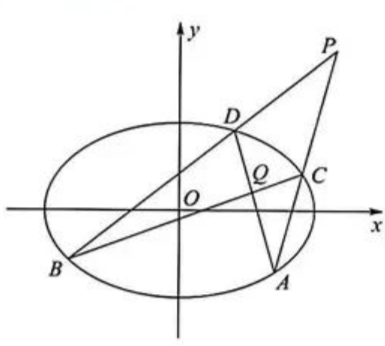
\includegraphics[width=0.5\textwidth]{flg/example.png} % 调整图片大小
    \par\vspace{1cm}
    {\small \copyright{} 2025 版权所有}
\end{titlepage}
% 前言部分
\frontmatter
\pagestyle{frontmatter} % 应用前言样式
% 前言内容
\chapter*{前言}
本书内容全部使用\LaTeX{}进行排版,作者"还在尬黑"是一位准大一学生,高中毕业于广东深圳中学,高三数学各次大考平均排名位于前5\%,高考应该也不例外。"还在尬黑"拥有知乎(同名),微信公众号(同名),小红书号(同名)等账号,头像是一个右手三叶结。以及不同名不同头像的GitHub账号,发表原创优质内容百余篇,在此十分感谢读者的支持和赞助!

"还在尬黑"对圆锥曲线的解题研究有着浓厚兴趣,并在书中将其总结成了一套完整的解析几何教程。本书适合高中解析几何解题体系未成熟的高二高三学生,以及前来自学的高一学生以及初中生,也可作为高中数学教材。笔者衷心希望本书能够帮助读者提高圆锥曲线解题速度和解题能力,并能够准确地识别班内的"大佬"是用什么东西来装逼的。
\begin{flushright}
    \vspace{2\baselineskip} % 在署名前留出两行空白
    \kt 还在尬黑 \\ % 楷体斜体
    \today
\end{flushright}
\begin{figure*}[htbp]
	\centering
    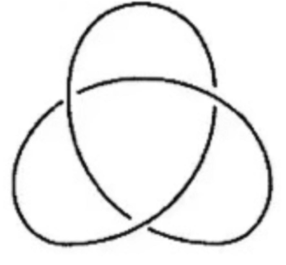
\includegraphics[width=0.25\textwidth]{flg/logo.png}%
	\caption{我的头像}
	\label{fig0-1}
\end{figure*}

% 目录部分(关键修改)
\newpage
\CTEXoptions[tocdepth=2] % 设置目录深度为章和节
\tableofcontents
\thispagestyle{tocmatter} 
% 正文部分
\mainmatter
\pagestyle{mainmatter} % 应用正文样式

% 章节内容
\chapter{先导课程}
\chaptermark{先导课程}
\section{写在前面}
解析几何是高中数学的重要学习内容,在高考中分值占比较高。

不少教辅会以“圆锥曲线”作为替代性的表述,这可能是因为圆锥曲线是解析几何中的重难点。但笔者认为“解析几何”更为贴切:第一,从应试角度考虑,圆锥曲线是解析几何的子集,现在考试有的题也会出直线和圆,新定义曲线(如3次曲线等)进行考察;第二,笔者打算从不单单只谈3种圆锥曲线,而是想在其基础之上,更多地普及一些考试常用的几何知识和背景;第三,笔者愿意先从最基本的直线开始说起,帮助读者搭建完整的解析几何体系。

首先,笔者来讲一讲怎么进行计算。这似乎是一个很简单的问题,但是谁又能保证在紧张刺激的考场环境下不会犯错误?一旦出现计算错误,检查就需要花费一定的时间,所以不如挑选合适的计算方法,从源头上减少失误。本节中,笔者会结合自己的一些实战经验,尽量告诉大家一些计算过程中减小失误,提升速度的技巧和方法,以及解析几何中计算的基本方向----整体代换。

鉴于本书的覆盖群体,笔者会尽量避免过多的公式推导和过于严谨的学术表述,而是从直观的角度出发,用一些具体的例子来说明计算的过程。希望大家能从中受益。
\section{轮换,对称}
在此之前,请允许我先介绍一些基本的概念,我们不妨先来看一些看起来很整齐的式子,这些式子平时很常见,大家在备考强基计划的过程中也会遇到比较多这样的式子:
\begin{example}{}{}
    观察以下代数式,并尝试在心里面归纳出它们的特点:\vspace{-10pt}
    \begin{gather*}
        abc\\
        a+b+c \\
        ab+bc+ca \\
        a^2+b^2+c^2 \\
        (a+b)(b+c)(c+a)\\
        a²b + a²c + b²a + b²c + c²a + c²b
    \end{gather*}
\end{example}
\begin{solution}
    相信大部分同学是通过自己的直觉来归纳的,直观的感受就是这些式子很“整齐”,而且很有规律可循。那么问题来了:“整齐”是怎么体现的?更进一步地,有没有手段验证一个代数式是“整齐”的?至于“很有规律可循”,那么规律是什么?
    
    这些问题循序渐进,如果理清这些问题,那么读者便掌握了学习数学时地最基本的关注点:定义,性质,判定。这些式子中的$a,b,c$​​结构权重是均等的​​,它们地位相同,没有“特权变量”,也没有“次序”之分。
    
    而且,眼尖的读者可以发现,这些表达式中的项往往成组出现​​,覆盖所有可能的组合,比如$a+b+c$中全为一次项,如果$a$出现了,不用猜也知道$b$和$c$也出现了;再比如$a²b + a²c + b²a + b²c + c²a + c²b$中,$a^2b$出现了,其中$a$被平方了,那不用猜也知道在其他的项中,$b$和$c$也会被平方,而且后面一定会跟着其他没有被平方的字母。它们出现的次数相同。
    
    {\heiti 事实上,由于乘法和加法的交换律和结合律,我们可以发现,对于上面任意一个式子,我们都可以挑选任意两个变量交换位置,而多项式本身保持不变。}大家不妨想象一下阅兵式的场景,即使我们偷偷调换两个兵的位置,你也看不出来有什么异样,这是阅兵队伍“整齐”的体现。同样地,这个代数式也可以这样操作,来验证这个代数式是“整齐”的,“规律可循”的。这样我们便可以引出对称式的概念。
\end{solution}
\begin{definition}{对称式}{}
    对于一个 $n$ 元多项式 $P(x_1, x_2, \dots, x_n)$,若对于数 $1, 2, \dots, n$ 的任意一个排列 $(i_1, i_2, \dots, i_n)$,都有
    \[
    P(x_{i_1}, x_{i_2}, \dots, x_{i_n}) = P(x_1, x_2, \dots, x_n),
    \]
    则称 $P(x_1, x_2, \dots, x_n)$ 为对称式。
\end{definition}
“对称”​​ 体现在字母地位平等,没有哪个字母是特殊的。只要式子中包含某个由特定字母组成的项(例如$a^2b$),那么它一定包含由所有其他字母以同样的方式组成的项(即$a^2c,b^2a,b^2c,c^2a,c^2b$)。

这样我们就认识了对称式的概念,这样当读者听到别人说“对称式”的时候,不会至于一脸懵逼,或者一边点头,假装听懂,然后用直觉去理解这个概念(这样的情况长期发展下去,是不利于学习数学的)。当然,读者也许会发现,像“$a²b + a²c + b²a + b²c + c²a + c²b$”这样的式子其实比较长,占用了较大的空间,也显得不够简洁。因此我们不妨规定以下记号:
\begin{definition}{循环和}{}

\end{definition}

\begin{property}{对称式的性质}{}
    (1)基本对称多项式的基础性​​:

\end{property}

那么下面我们乘胜追击,再来看一组式子:
\begin{example}{}{}
    观察以下代数式,并尝试在心里面归纳出它们的特点:\vspace{-10pt}
    \begin{gather*}
        a^2b+b^2c+c^2a\\
        a^3b+b^3c+c^3a\\
        \dfrac{a}{b+c}+\dfrac{b}{c+a}+\dfrac{c}{a+b}
    \end{gather*}
\end{example}
\begin{solution}
    和刚才的对称式不同,如果我们这里调换某两个字母的位置,那么结果也会发生变化。比如$a^2b+b^2c+c^2a$中,如果我们把$a$和$b$调换位置,那么结果也会发生变化,比如说新出现了$b^2a$项,这是原来所没有的。

    但是读者会发现,这个式子看上去也是有规律可循的,比如$a^3b+b^3c+c^3a$中,$a^3$项出现了,那不用猜也知道$b^3$和$c^3$也会在其它部分出现,而且出现的次数相同,但是和上文的规律不一样,$a^3$后面只会跟着$b$,却没有$c$,即没有$a^2c$项。
\end{solution}
\begin{example}{}{}
    将$(a+b)(b+c)(c+a)$进行展开,并尽己所能地保证结果的每个部分都是由$a,b,c$三个元同时出现且地位相同的式子:
\end{example}
\begin{solution}
    先展开,再重组:\vspace{-10pt}
    \begin{align*}
    \vspace{-15pt}
    (a+b)(b+c)(c+a)&=(b^2+ac+ab+bc)(a+c)\\
    &=ab^2+b^2c+a^2c+ac^2+a^2b+abc+abc+bc^2\\
    &=(a+b+c)(ab+bc+ca)-abc
    \vspace{-10pt}
    \end{align*}
\end{solution}
最后为什么

\begin{theorem}{}{}
    $$(a+b)^2=a^2+2ab+b^2$$

\end{theorem}
% 第二章:导数与微分
\chapter{导数与微分}
\section{导数的定义}
\begin{example}{}{}
    已知$x,y>0$,且$x^2+9y^2=12$,则$\dfrac{x+2}{y+1}-3x$的最小值为\underline{\hspace{2cm}}.
\end{example}
\begin{solution}

\end{solution}
\begin{example}{}{}
    (单选)数列$a_{n}$各项为正整数且递增,$a_{n+2}=C_{a_{n+1}}^{a_{n}}$,则(~~~~~)

    \begin{tabular}{@{}ll@{}}
        A.$a_n<a_{n-1}+1$&B.$a_1,a_2,a_3$可能成等比数列\\
        C.$a_3a_4<a_5$&D.$a_3,a_4,a_5$可能成等比数列
    \end{tabular}
\end{example}
\begin{solution}
由于$a_n$递增,则A显然错误;下面考虑选项BD:
\[
    a_na_{n+2} = a_nC_{a_{n+1}}^{a_{n}}=a_{n+1}C_{a_{n+1}-1}^{a_{n}-1}=a_{n+1}^2\\\Rightarrow a_{n+1}=C_{a_{n+1}-1}^{a_{n}-1}
\]

当$a_n=1$时,代入表达式得到$a_{n+1}=C_{a_{n+1}-1}^{0}=1=a_n$,与数列递增矛盾;

当$a_n=2$时,代入表达式得到$a_{n+1}=C_{a_{n+1}-1}^{1}=a_{n+1}-1<a_{n+1}$,矛盾;

当$a_n>2$时,易得$a_{n+1}-1>2$,代入表达式得到
\[a_{n+1}=C_{a_{n+1}-1}^{a_{n}-1}\ge C_{a_{n+1}-1}^{2}=\dfrac{(a_{n+1}-1)(a_{n+1}-2)}{2}\]

解方程发现无整数解,而且由于$C_{a_{n+1}-1}^{1}=a_{n+1}-1$是小于$a_{n+1}$的最大整数,且有

\[C_{a_{n+1}-1}^{1}<C_{a_{n+1}-1}^{2},~~C_{a_{n+1}-1}^{2}\ne a_{n+1}\]

只可能是$C_{a_{n+1}-1}^{2}> a_{n+1}$.

雪上加霜的是,$C_{a_{n+1}-1}^{2}$和$C_{a_{n+1}-1}^{1}$中间没有数可以等于$C_{a_{n+1}-1}^{m}$,所以BD错误;

考虑C,易得$a_1\ne1,a_2\ge 4,a_3\ge6,a_4=C_{a_3}^{a_2}>2a_3+1$,由
\[a_5=C_{a_4}^{a_3}>a_3a_4 \Rightarrow a_3^2<C_{a_{4}-1}^{a_{3}-1}<C_{2a_3}^{a_3-1}\]

转化为$a_3^3+a_3<C_{2a_3}^{a_3}$这是显然成立的,故本题目选C
\end{solution}
\begin{example}{}{}
    已知$\triangle{ABC}$中,$A=3B=9C$,则$\cos A\cos B+\cos B\cos C+\cos C\cos A=$\underline{\hspace{1cm}}.
\end{example}
\begin{solution}
解得$A=\dfrac{9\pi}{13},B=\dfrac{3\pi}{13},C=\dfrac{\pi}{13}$考虑积化和差:
\begin{align*}
&\cos A\cos B+\cos B\cos C+\cos C\cos A\\
&=\dfrac12(\cos(A+B)+\cos(A-B)+\cos(B+C)+\cos(B-C)+\cos(A+C)+\cos(A+C))\\
&=\dfrac12(\cos\dfrac{12\pi}{13}+\cos\dfrac{6\pi}{13}+\cos\dfrac{4\pi}{13}+\cos\dfrac{2\pi}{13}+\cos\dfrac{10\pi}{13}+\cos\dfrac{8\pi}{13})\\
&=\dfrac{1}{2\sin\dfrac{\pi}{13}}\sin\dfrac{\pi}{13}(\cos\dfrac{2\pi}{13}+\cos\dfrac{4\pi}{13}+\cos\dfrac{6\pi}{13}+\cos\dfrac{8\pi}{13}+\cos\dfrac{10\pi}{13}+\cos\dfrac{12\pi}{13})\\
&=\dfrac{1}{4\sin\dfrac{\pi}{13}}(\sin\dfrac{\pi}{13}-\sin\dfrac{3\pi}{13}+\sin\dfrac{3\pi}{13}-\sin\dfrac{5\pi}{13}+\sin\dfrac{5\pi}{13}-\sin\dfrac{7\pi}{13}\\
&~~~~~~~~~~~~~~~~+\sin\dfrac{7\pi}{13}-\sin\dfrac{9\pi}{13}+\sin\dfrac{9\pi}{13}-\sin\dfrac{11\pi}{13}+\sin\dfrac{11\pi}{13}-\sin\dfrac{13\pi}{13})\\
&=-\dfrac14
\end{align*}
\end{solution}
% 图片插入示例(注释掉,避免报错)
% \begin{figure}[htbp]
%     \centering
%     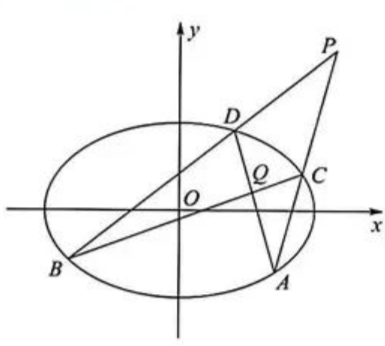
\includegraphics[width=0.6\textwidth]{flg/example.png}
%     \caption{导数的几何意义}
%     \label{fig:derivative}
% \end{figure}

\end{document}